\documentclass[11pt,a4paper]{article}
\usepackage[utf8x]{inputenc}
\usepackage[T1]{fontenc}
\usepackage{graphicx}
\usepackage[usenames, dvipsnames]{color}
\usepackage{fancyhdr}
\usepackage{datetime}
\setlength{\headheight}{15.2pt}
\pagestyle{fancy}
\fancyhf{}

\lhead{\textbf{\Large\color{MidnightBlue}Design and Modelling of Software Systems 
    \hfill Page: \thepage \\ ETFOS, 2011}}

\setlength{\parindent}{0cm}

\begin{document}
\large
Laboration Assignment No. 5\\
Submission Date - \yyyymmdddate \today \\
Damir, Jelić, damir.jelic@etfos.hr \\
Marijan, Svalina, msvalina@etfos.hr
\\
\rule{\linewidth}{0.1mm}
\setcounter{section}{5}
\subsection{KWIC use case diagram}
\begin{description}
    \item[Actors:] \hfil
    \begin{itemize}
    \item
        Librarian
        \begin{description}
            \item[] Librarian is an actor who is in charge of generating KWIC data.
        \end{description}
    \end{itemize}

    \item[Use cases:] \hfil
        \begin{description}
            \item[Name:] Generate KWIC data
            \item[Initiator:] Librarian
            \item[Goal:]The Librarian wants to generate keywords for one particular context
                 \begin{enumerate}
                    \item The librarian enters a number of titles
                    \item The librarian enters an empty title 
                    (to indicate that all titles have been entered) 
                    \item The system outputs an alphabetically sorted list 
                    of all circular shifts of all the titles
                 \end{enumerate}
        \end{description}
        \item[Use Case Diagram:] \hfil
\end{description}
     \begin{figure}[htb]
         \begin{center}
             \setlength\fboxsep{0pt}
             \fbox{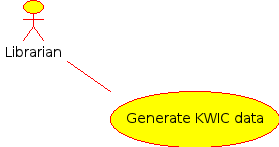
\includegraphics[scale=1]{use_case.png}}
             \caption{Simple use case diagram}
             \label{fig:class_diag}
        \end{center}
    \end{figure}

\newpage
\subsection{KWIC class diagram}
     \begin{figure}[htb]
         \begin{center}
             \setlength\fboxsep{0pt}
             \fbox{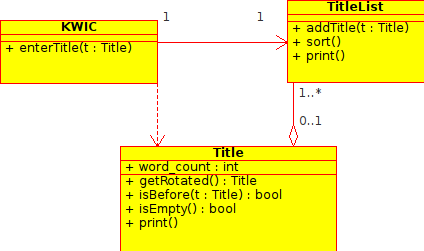
\includegraphics[scale=1]{class_diagram.png}}
             \caption{Class diagram}
             \label{fig:class_diag}
        \end{center}
    \end{figure}
\begin{description}
   \begin{itemize}
        \item getRotated()
            \begin{description}
                Returns a copy of the title, after one circural shift.
            \end{description}
         \item isBefore()
            \begin{description}
                Returns true if the title is alphabetically before the argument title.
            \end{description}
        \item isEmpty()
            \begin{description}
                Returns true if the title is empty.
            \end{description}

  \end{itemize}

\end{description}

\newpage
\subsection{KWIC sequance diagram}
    \begin{figure}[htb]
       \begin{center}
             \setlength\fboxsep{0pt}
             \fbox{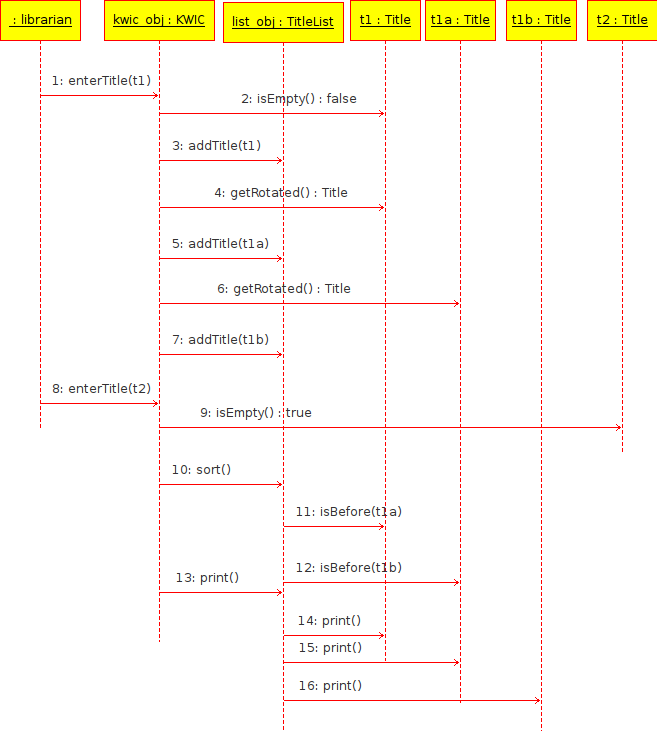
\includegraphics[scale=0.76]{sequence_diagram.png}}
             \caption{Sequence diagram}
             \label{fig:class_diag}
       \end{center}
    \end{figure}
\begin{description}
   \begin{itemize}
            \begin{description}
                Afrer Labrarian enters first title, isEmpty() function is called. Since
                its not empty the title is added to the list.
                Title then gets rotatetd and all combinations are added to the list.
                After second empty title is enterd, list is sorted and then printed.
                
            \end{description}
\end{description}


\end{document}
